\documentclass[spanish, aspectratio=169]{beamer}

\usepackage{graphicx}
\usepackage{subcaption}
\graphicspath{ {figures/} }


\begin{document}
	
	
\frame{\titlepage}

\begin{frame}{Motivation}
	\vspace{-0.5cm}
	\begin{block}{}
		Mental disorders affect cognition, behavior, and emotions of millions of people worldwide. Around 350 million individuals suffer from a mental disorder \cite{Dehghan-Bonari2023}.
	\end{block}
	
	\begin{columns}
		\small
		\vspace{-0.2cm}
		\column{0.33\textwidth}
		\centering
		\includegraphics[width=0.5\textwidth]{figures/OppositionalDefiantDisorder.png}
		
		\vspace{0.5em}
		\textbf{Oppositional Defiant Disorder}
		
		\column{0.33\textwidth}
		\centering
		\includegraphics[width=0.5\textwidth]{figures/BipolarDisorder.png}
		
		\vspace{0.5em}
		\textbf{Bipolar Disorder}
		
		\column{0.33\textwidth}
		\centering
		\includegraphics[width=0.5\textwidth]{figures/ADHD.png}
		
%		\vspace{0.5em}
		\textbf{Attention Deficit Hyperactivity Disorder}
	\end{columns}
%	\vspace{-0.5cm}
	\pause
	\begin{block}{Challenges:}
		lengthy follow-up, subjective interpretations, inefficient criteria, and limited access to clinical care.
	\end{block}
	
\end{frame}

\begin{frame}{Problem Statement and Research Question}
	
\renewcommand{\arraystretch}{1.5} 

\begin{table}[htbp]
	\centering
	\footnotesize
	\begin{tabular}{>{\raggedright\arraybackslash}p{3.1cm} >{\centering\arraybackslash}p{2cm} >{\centering\arraybackslash}p{2cm} >{\centering\arraybackslash}p{2cm} >{\centering\arraybackslash}p{2cm}}
		\toprule
		\diagbox{\textbf{Model}}{\textbf{Challenge}} & \textbf{Complex Patterns} & \textbf{High Labeled Data Volume} & \textbf{Stochasticity} & \textbf{Data Shift} \\
		\midrule
		Machine Learning \cite{Salari2023} & \textcolor{purple}{\ding{55}} & \textcolor{teal}{\ding{51}} & \textcolor{teal}{\ding{51}} & \textcolor{purple}{\ding{55}} \\[1mm]
		Deep Learning  \cite{LOHANI2023111689}    & \textcolor{teal}{\ding{51}}    & \textcolor{purple}{\ding{55}} & \textcolor{teal}{\ding{51}} & \textcolor{teal}{\ding{51}} \\[1mm]
		Foundation \cite{Sibley21042021}                   & \textcolor{teal}{\ding{51}}    & \textcolor{teal}{\ding{51}}    & \textcolor{purple}{\ding{55}} & \textcolor{teal}{\ding{51}} \\
		\bottomrule
	\end{tabular}

\end{table}

\pause	
	
	\begin{block}{Research Question}
		\footnotesize
		How to develop a stochastic foundational model for inference from biological signals that integrates Gaussian processes to support clinical practice through EEG signal analysis, considering the variability and inconsistencies present in the datasets?
	\end{block}	
\end{frame}



\begin{frame}{Objectives}
%	\vspace{-0.3cm}
	\begin{block}{General Objective}
		\small
		Develop a stochastic learning methodology related to EEG recordings based on a foundational model that integrates labeled and unlabeled databases using self-learning and fine-tuning techniques.
	\end{block}
	
	\vspace{-0.1cm}
	\begin{block}{Specific Objectives}
		\small
		\begin{enumerate}
			\item Develop a foundational model for the classification of biological signals related to EEG recordings, leveraging \textcolor{MyAccent}{unlabeled data} during the self-learning phase and labeled data for fine-tuning.
			\item Implement a \textcolor{MyAccent}{stochastic prediction} tool based on Gaussian processes to model uncertainty in the foundational model's predictions.
			\item Design a strategy to \textcolor{MyAccent}{manage variability and inconsistency} in EEG recording datasets, enabling the effective integration of databases with diverse standards.
		\end{enumerate}
	\end{block}
\end{frame}




\section{The Dataset}

\begin{frame}{Problem Setting}
	\begin{block}{}
		We define the multimodal input space as the Cartesian product of $P$ modality-specific input spaces:
		\[
		\mathcal{X} = \prod_{p=1}^{P} \mathcal{X}^{(p)},
		\]
		where each modality $\mathcal{X}^{(p)}$ may represent data from distinct sources.
	\end{block}
	
\end{frame}



\begin{frame}{Toadstool 2 Dataset}
\begin{block}{}
The dataset consists of video, sensor, and demographic data collected from 10 participants playing a Super Mario Bros.
\end{block}

\begin{block}{}
	We focus on sensor data. We get a total of 20970 samples corresponding to a label taking in a 4s time window.
\end{block}
		\begin{columns}[T] % Top alignment
		\begin{column}{0.5\textwidth}
			\begin{center}
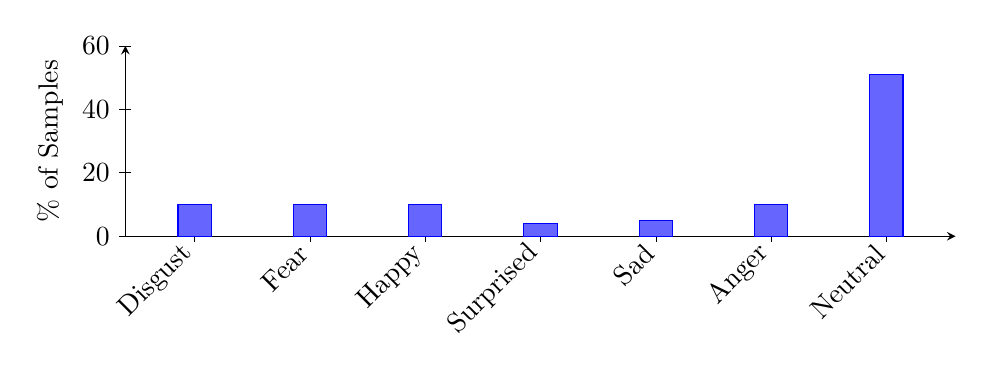
\begin{tikzpicture}
	\begin{axis}[
		width=\textwidth,
		height=4cm,
		ybar,
		bar width=12pt,
		axis lines=left,
		ylabel={\% of Samples},
		symbolic x coords={Disgust,Fear,Happy,Surprised,Sad,Anger,Neutral},
		xtick=data,
		xticklabel style={rotate=45, anchor=east},
		ymin=0, ymax=60,
		tick style={black},
		enlarge x limits=0.1  % adds horizontal margin on both sides
		]
		\addplot+[fill=blue!60] coordinates {
			(Disgust,10) (Fear,10) (Happy,10)
			(Surprised,4) (Sad,5) (Anger,10) (Neutral,51)
		};
	\end{axis}
\end{tikzpicture}

			\end{center}
			
		\end{column}
		\begin{column}{0.5\textwidth}

%		\vspace{0.5em}
		\centering
		\small
		\begin{tabular}{lcc}
		\toprule
		\textbf{Signal} & \textbf{Rate (Hz)} & \textbf{Channels} \\
		\midrule
		BVP  & 64 & 1      \\
		ACC  & 32 & 3 		\\
		EDA  & 4  & 1      \\
		HR   & 1  & 1      \\
		\bottomrule
		\end{tabular}
		



		\end{column}
	\end{columns}
\end{frame}


\begin{frame}{Total Class Distribution (\% of Samples)}
	\begin{center}
		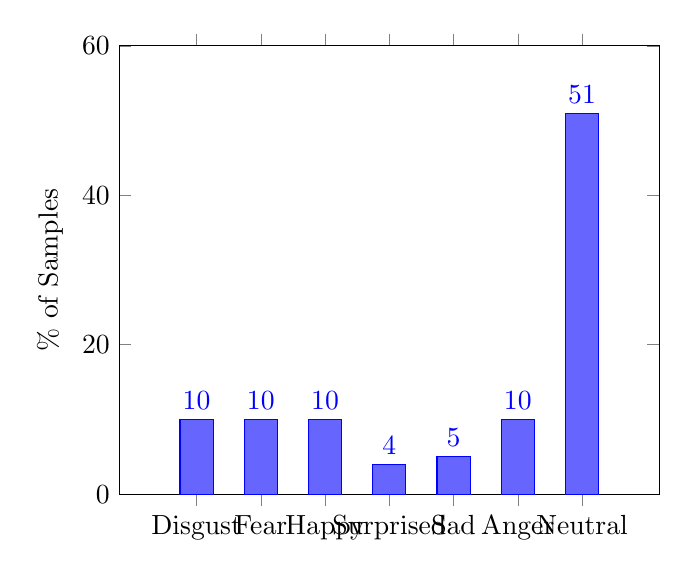
\begin{tikzpicture}
			\begin{axis}[
				ybar,
				bar width=12pt,
				enlarge x limits=0.2,
				ylabel={\% of Samples},
				symbolic x coords={Disgust,Fear,Happy,Surprised,Sad,Anger,Neutral},
				xtick=data,
				nodes near coords,
				nodes near coords align={vertical},
				ymin=0, ymax=60
				]
				\addplot+[fill=blue!60] coordinates {
					(Disgust,10) (Fear,10) (Happy,10) (Surprised,4) (Sad,5) (Anger,10) (Neutral,51)
				};
			\end{axis}
		\end{tikzpicture}
	\end{center}
\end{frame}



\section[Predicting the dispatch of thermoelectric generation]
{Predicting the dispatch of thermoelectric generation}


\begin{frame}{Problem Setting}
	
	
	Consider a vector collecting sequential data across $P$ variables at time instant \( t \), as \( \boldsymbol{v}_t \subseteq \mathbb{R}^{P}\). The flattening of \( T \) sequential observations yields an input vector \( \boldsymbol{x} \in \mathcal{X} \),
	
	
	\[ 
	\boldsymbol{x}= [ \boldsymbol{v}_{t-1}^\top, \boldsymbol{v}_{t-2}^\top, \cdots, \boldsymbol{v}_{t-T}^\top  ]^\top,
	\]
	
	
	\( {\mathcal{X}} \subseteq \mathbb{R}^{L} \), and \( L = PT \). The forecasting task aims to predict the next \(H\) sequential values, yielding the output target \( \boldsymbol{y} \in {\mathcal{Y}} \)
	
	
	\[
	\boldsymbol{y} = [ \boldsymbol{v}_{t}^\top, \boldsymbol{v}_{t+1}^\top, \cdots, \boldsymbol{v}_{t+H-1}^\top  ]^\top,
	\] 
	
	
	\( {\mathcal{Y}} \subseteq \mathbb{R}^{D} \), and \( D = PH \). Gathering \( N \) input-output i.i.d. observation pairs produces the training dataset as \( {\mathcal{D}} = \{\boldsymbol{x}_n, \boldsymbol{y}_n\}_{n=1}^N = \{ \boldsymbol{X}, \boldsymbol{Y}\} \).
	
	
\end{frame}


\begin{frame}{The Chained Model}
	
	For dataset $\mathcal{D}$, the likelihood function assumes the distribution over \(  \boldsymbol{Y} \) as the product of \( D \) conditionally independent distributions, one by each output as follows:
	
	
	\[
	p(\boldsymbol{Y} \mid \boldsymbol{\theta}(\boldsymbol{X})) = \prod_{n=1}^N \prod_{d=1}^D p\left(y_{n,d} \mid \boldsymbol{\theta}_d(\boldsymbol{x}_n)\right),
	\]
	
	
	where \( \boldsymbol{\theta}(\boldsymbol{X}) = \{ \boldsymbol{\theta}_d(\boldsymbol{x}_n) \}_{n=1,d=1}^{N, D} \), with \( \boldsymbol{\theta}_d(\boldsymbol{x}) \subseteq \mathbb{R}^{J_d} \) as a vector containing \( J_d \) parameters for \( d \)-th output distribution with elements \( \theta_{d,j}(\boldsymbol{x}) \). \emph{Each likelihood parameter is governed by a Gaussian Process (GP) \( f_{d,j}(\boldsymbol{x}) \)} via a link function transformation \( h_{d,j}(\cdot) \) as \( \theta_{d,j}(\boldsymbol{x}) = h_{d,j}(f_{d,j}(\boldsymbol{x})) \).
	
\end{frame}

\begin{frame}{The LMC Model}
	
	Consider a set of \( Q \) zero-mean independent GPs \( \{ g_q \}_{q=1}^Q \) with kernel function \(k_q(\boldsymbol{x}, \boldsymbol{x}')\) that will be linearly weighed via \( a_{(d,j),q} \in \mathbb{R} \) coefficients to generate \( f_{d,j} \) as
	
	\[
	f_{d,j}(\boldsymbol{x}) = \sum_{q=1}^Q a_{(d,j),q} g_{q}(\boldsymbol{x}),
	\]
	
	proposing a \emph{cross-covariance function for the latent variables \( f_{d,j} \)} as follows
	
	\[
	k_{\boldsymbol{f}_{d,j}, \boldsymbol{f}_{d',j'}}(\boldsymbol{x}, \boldsymbol{x}') = \text{cov}\{f_{d,j}(\boldsymbol{x}), f_{d',j'}(\boldsymbol{x}')\}
	=\sum_{q=1}^Q a_{(d,j),q}a_{(d',j'),q} k_{q}(\boldsymbol{x}, \boldsymbol{x}').
	\]
	
	We call the above as Linear Model of Coregionalization (LMC).
	
\end{frame}

\begin{frame}{Variational Optimization}
	
	
	We introduce induced vectors \( \mathbf{u} \in \mathbb{R}^{MQ} \) with elements \( g_q(\mathbf{z}_m) \) at	\( M \ll N \) inducing points \( \{\mathbf{z}_m\}_{m=1}^M \) to reduce the complexity \emph{\(\mathcal{O}(N^3)\) to \(\mathcal{O}(NM^2)\)}, and approximating the joint posterior
	
	
	\[
	p(\mathbf{f},\mathbf{u}\mid \mathcal{D}) 
	\approx \prod_{d=1}^D \prod_{j=1}^{J_d} p(\mathbf{f}_{d,j}\mid \mathbf{u})
	\prod_{q=1}^Q q(\mathbf{u}_q),
	\]
	
	
	with \( q(\mathbf{u}_q)=\mathcal{N}(\mathbf{u}_q\mid \boldsymbol{\mu}_q,\mathbf{S}_q) \), \( \boldsymbol{\mu}_q \in \mathbb{R}^{M} \), \( \boldsymbol{S}_q \in \mathbb{R}^{M \times M} \), and \( \boldsymbol{f}_{d,j} = [f_{d,j}(\boldsymbol{x}_1), \cdots, f_{d,j}(\boldsymbol{x}_N) ]^\top \in \mathbb{R}^{N} \).
	We tune the model by optimizing the loss function \(\mathcal{L}\)
	
	
	\[
	\mathcal{L} = \sum_{n=1}^{N}\sum_{d=1}^{D}
	\mathbb{E}_{q(\mathbf{f}_{d,n})}\!\left\{\log p(y_{d,n}\mid f_{d,1}(\mathbf{x}_n), \cdots, f_{d,J_d}(\mathbf{x}_n))\right\}
	- \sum_{q=1}^{Q}\mathrm{KL}\!\left\{q(\mathbf{u}_q)\parallel p(\mathbf{u}_q)\right\},
	\]
	
	
	using  Natural Gradient for \(\mathbf{u}_q\) and \(\mathbf{\boldsymbol{S}}_q\), and Adam for the remaining parameters~\cite{pmlr-v84-salimbeni18a}.
	
\end{frame}


\begin{frame}{Linear Hydrothermal Dispatch Model}
	Thermal demand can be predicted from hydrological resources by solving a 
	hydrothermal dispatch problem. In its simplest form, it is modeled as a 
	linear optimization problem:
	
	\vspace{0.5em}
	
	
	\begin{columns}[c,onlytextwidth]
		% --- Left column: equations ---
		\column{0.48\textwidth}
		\begin{gather*}
			\min_{E_T} \;\; \sum_{i=1}^{N_T} \eta_i E_{T,i}\\[0.5em]
			\text{s.t. } \; E_{H,j} = V_{j,t} - V_{j,t+1} + A_{j,t}\\[0.5em]
			\sum_{i=1}^{N_T} E_{T,i} = E_D - \sum_{j=1}^{N_H} E_{H,j}\\[0.5em]
			E_{T,i}^{\min} \leq E_{T,i} \leq E_{T,i}^{\max}
		\end{gather*}
		
		\footnotesize
		\column{0.52\textwidth}
		\begin{itemize}
			\item $E_T$: Thermal generation
			\item $E_H$: Hydropower generation
			\item $E_D$: Daily demand
			\item $N_T, N_H$: Number of thermal/hydro plants
			\item $\eta_i$: Heat rate of thermal plant $i$
			\item $V$: Reservoir volume
			\item $A$: Reservoir inflow
			\item $t$: Time index
			\item $E_{T}^{\min}, E_{T}^{\max}$: Thermal limits
		\end{itemize}
	\end{columns}
\end{frame}
\section[Design an optimization strategy for long term planning]{Design an optimization strategy for long term planning}

\begin{frame}{Nodes}
	A node represents an interconnection point of different elements of the gas network where their flows converge.
	
	\begin{columns}[c,onlytextwidth] 

		\column{0.55\textwidth}
		\centering
		\includegraphics[width=\textwidth]{estructura_nodo}
		
		\column{0.4\textwidth}
		\begin{itemize}
			\item [$f_{iny}$] Injected flow.
			\item [$f_{dem}$] Demanded flow.
			\item [$f_{rest}$] Equivalent restoration flow of unmet demand.
			\item [$f_{N}$] Flow within the network (net flow).
		\end{itemize}
	\end{columns}
\end{frame}


\begin{frame}{Pipelines}
	Pipelines are the physical infrastructure through which gas is transported. They are characterized by the pair of nodes they connect and by their gas transport capacities. 
	
	\centering
	\includegraphics[width=0.6\textwidth]{estructura_gasoducto}
	
	\begin{itemize}
		\item [$f_{i,j}$] Flow transported through the pipeline.
		\item [$p_{i}$] Pressure at the suction node.
		\item [$p_{j}$] Pressure at the discharge node.
	\end{itemize}
	
\end{frame}


\begin{frame}{Compressors}
	Compressors, like pipelines, are elements that interconnect pairs of nodes and transport a flow of gas. Their role in the system is to increase the pressure at the discharge node relative to the suction node in order to transport gas over longer distances and compensate for pressure losses due to friction in the pipelines.
	
	\begin{columns}[c,onlytextwidth] 
		
		\column{0.4\textwidth}
		\begin{itemize}
			\item [$f_{i,j}$] Flow transported through the compressor.
			\item [$p_{i}$] Pressure at the suction node.
			\item [$p_{j}$] Pressure at the discharge node.
		\end{itemize}
		
		
		\column{0.55\textwidth}
		
		\centering
		\includegraphics[width=\textwidth]{estructura_compresor}
	\end{columns}
\end{frame}


\begin{frame}{Loss Function}
	The loss function represents the objective to be minimized in the optimization model. 
	It quantifies the total operational cost of the natural gas network, 
	combining injection, transport, compressor operation, and unmet demand costs.
	
	\[
	\mathcal{L} = 
	\sum_{w \in \mathcal{W}} \emph{C_{\text{iny}}^w f_{\text{iny}}^w} \;+\;
	\sum_{p \in \mathcal{P}} C_{\text{trans}}^p f_{\text{trans}}^p \;+\;
	\sum_{c \in \mathcal{C}} C_{\text{trans}}^c f_{\text{trans}}^c \;+\;
	\sum_{i \in \mathcal{N}} \sum_{u \in \mathcal{U}} C_{\text{rest}}^{u,i} f_{\text{rest}}^{u,i}
	\]
	  Each component is defined as the product of a unit cost and the corresponding flow:
	\begin{columns}[T,onlytextwidth] 
		
		\column{0.48\textwidth}
		\begin{itemize}
			\item Injection at node $w$: $C_{\text{iny}}^w \, f_{\text{iny}}^w$
			\item Transport through pipeline $p$: $C_{\text{trans}}^p \, f_{\text{trans}}^p$
		\end{itemize}
		
		\column{0.48\textwidth}
		\begin{itemize}
			\item Transport through compressor $c$: $C_{\text{trans}}^c \, f_{\text{trans}}^c$
			\item Unmet demand for user $u$ at node $i$: $C_{\text{rest}}^{u,i} \, f_{\text{rest}}^{u,i}$
		\end{itemize}
	\end{columns}
	

\end{frame}

\section[\empty]{Objective 3: Long Short-Term Memory (LSTM) Architecture}

\begin{frame}{Transformer and Attention Mechanism}
	\begin{columns}[c] % [c] = vertically center
		
		% Left column
		\begin{column}{0.48\textwidth}
			\centering
			\scalebox{0.5}{
\begin{tikzpicture}[
	>=LaTeX, % Use default LaTeX arrows
	very thick,
	arrow/.style={
		-latex,
		very thick,
		rounded corners=0.2cm
	},
	block/.style={
		rectangle,
		fill=gray!10,
		rounded corners=3mm,
		draw,
		very thick
	},
	layer/.style={
		rectangle,
		fill=white!10,
		rounded corners=1mm,
		inner xsep=0em,
		inner ysep=0.25em,
		minimum height=1.4em,
		align=center,
		text width=2.5cm,
		draw,
		very thick
	},
	input/.style={ % Input or output node
		circle,
		minimum width=2.25em,
		draw,
		fill=gray!10,
		thick
	},
	do path picture/.style={%
		path picture={%
			\pgfpointdiff{\pgfpointanchor{path picture bounding box}{south west}}%
			{\pgfpointanchor{path picture bounding box}{north east}}%
			\pgfgetlastxy\x\y%
			\tikzset{x=\x/2,y=\y/2}%
			#1
		}
	},
	sin wave/.style={do path picture={    
			\draw [line cap=round] (-3/4,0)
			sin (-3/8,1/2) cos (0,0) sin (3/8,-1/2) cos (3/4,0);
		}
	}
	]
	
	\node[input] (iemb) at (1.25,-0.45) {$\mathbf{x}$};
	\node[input] (oemb) at (5.25,-0.45) {$\mathbf{y}$};
	
	% Sums
	\node[circle, draw, minimum size=0.25em, inner sep=0pt, above=1em of iemb] (sum1) {$\mathbf{+}$};
	\node[circle, draw, minimum size=0.25em, inner sep=0pt, above=1em of oemb] (sum2) {$\mathbf{+}$};
	% Positional Encoding
	\node [circle, draw, sin wave, minimum size=2em, left=0.8em of sum1] (pe1) {};
	\node [circle, draw, sin wave, minimum size=2em, right=0.8em of sum2] (pe2) {};
	
	% Encoder, 1st layer
	\node[layer] (add1) at (1.25,3.43) {Add \& Norm};
	\node[layer] (attn1) at (1.25,2.58) {Multi-Head \vspace{-0.05cm} \linebreak Attention};
	\draw[] (attn1) -- (add1);
	% Encoder 2nd sub-layer
	\node[layer] (add4) at (1.25,5.98) {Add \& Norm};
	\node[layer] (ff1) at (1.25,5.13) {Feed \vspace{-0.05cm} \linebreak Forward};
	\draw[] (ff1) -- (add4);
	
	% Decoder 1st sub-layer
	\node[layer] (add3) at (5.25,3.83) {Add \& Norm};
	\node[layer] (attn3) at (5.25,2.78) {Masked \vspace{-0.05cm} \linebreak Multi-Head \vspace{-0.05cm} \linebreak Attention};
	\draw[] (attn3) -- (add3);
	% Decoder, 2nd sub-layer
	\node[layer] (add2) at (5.25,6.38) {Add \& Norm};
	\node[layer] (attn2) at (5.25,5.53) {Multi-Head \vspace{-0.05cm} \linebreak Attention};
	\draw[] (attn2) -- (add2);
	% Decoder 3rd sub-layer
	\node[layer] (add5) at (5.25,8.93) {Add \& Norm};
	\node[layer] (ff2) at (5.25,8.08) {Feed \vspace{-0.05cm} \linebreak Forward};
	\draw[] (ff2) -- (add5);
	
	\coordinate (d1) at ($(attn3.south east) + (0.75,-0.7)$);
	\coordinate (d2) at ($(add5.north west) + (-0.15,0.05)$);
	\coordinate (e1) at ($(attn1.south east) + (0.15,-0.7)$);
	\coordinate (e2) at ($(add4.north west) + (-0.75,0.05)$);
	\begin{scope}[on background layer]
		\node[block, fit=(d1) (d2)] (decoder) {};
		\node[block, fit=(e1) (e2)] (encoder) {};
	\end{scope}
	
	% Classifier
	\node[layer, above=1.5em of add5] (linear) {Linear};
	\node[layer, above=1em of linear] (softmax) {Softmax};
	\node[input, above=1em of softmax] (probs) {$\hat{\mathbf{y}}$};
	
	\draw[arrow] (add1) -- (ff1);
	\draw[arrow] (add2) -- (ff2);
	\draw[arrow] (add5) -- (linear);
	\draw[arrow] (linear) -- (softmax);
	\draw[arrow] (iemb) -- (sum1);
	\draw[arrow] (sum1) -- (attn1);
	\draw[arrow] (oemb) -- (sum2);
	\draw[arrow] (sum2) -- (attn3);
	\draw[] (sum1) -- (pe1);
	\draw[] (sum2) -- (pe2);
	
	\draw[arrow] (ff1.south)++(0, -0.6) -| ($(add4.west) + (-0.6,-0.5)$) |- (add4.west);
	\draw[arrow] (attn1.south)++(0, -0.6) -| ($(add1.west) + (-0.6,-0.5)$) |- (add1.west);
	
	\draw[arrow] (attn3.south)++(0, -0.6) -| ($(add3.east) + (0.6,-0.5)$) |- (add3.east);
	\draw[arrow] (attn2.south)++(0, -0.6) -| ($(add2.east) + (0.6,-0.5)$) |- (add2.east);
	\draw[arrow] (ff2.south)++(0, -0.6) -| ($(add5.east) + (0.6,-0.5)$) |- (add5.east);
	
	\draw[arrow] (attn1.south)++(0, -0.4) -| ($(attn1.south) + (-1,0)$);
	\draw[arrow] (attn1.south)++(0, -0.4) -| ($(attn1.south) + (1,0)$);
	
	\draw[arrow] (attn3.south)++(0, -0.4) -| ($(attn3.south) + (-1,0)$);
	\draw[arrow] (attn3.south)++(0, -0.4) -| ($(attn3.south) + (1,0)$);
	
	\draw[arrow] (add4.north) |- ($(add4.north) + (1,1)$) -| ($(add4.north) + (2,-1)$) |- ($(attn2.south) + (-1,-0.4)$) -| ($(attn2.south) + (-1,0)$);
	\draw[arrow] (add4.north) |- ($(add4.north) + (1,1)$) -| ($(add4.north) + (2,-1)$) |- ($(attn2.south) + (0,-0.4)$) -| ($(attn2.south)$);
	\draw[arrow] (add3.north) |- ($(attn2.south) + (0.5,-0.4)$) -| ($(attn2.south) + (1,0)$);
	
%	\node[] at ($(oemb.east) + (1.4,0)$) {(shifted right)};
	\node[] at ($(pe1.west) + (-0.3,0)$) {$\mathbf{P}$};
	\node[] at ($(pe2.east) + (0.3,0)$) {$\mathbf{P}$};
	
	\draw[arrow] (iemb) -- (sum1);
	\draw[arrow] (oemb) -- (sum2);
	\draw[arrow] (softmax) -- (probs);
	
	\node[anchor=east] at ($(encoder.west) + (-0.2,0)$) {$N\times$};
	\node[anchor=west] at ($(decoder.east) + (0.2,0)$) {$N\times$};
\end{tikzpicture}
}
		\end{column}
		
		% Right column
		\begin{column}{0.48\textwidth}
			\centering
			\scalebox{0.7}{\input{figures/multihead_attention.tex}}
		\end{column}
		
	\end{columns}
\end{frame}

%\begin{frame}{Objective 3: Long Short-Term Memory (LSTM) Architecture}
%\begin{columns}[t]
%\begin{column}{0.65\textwidth}
%
%
%\begin{tikzpicture}[
%	% GLOBAL CFG
%	font=\sf \scriptsize,
%	>=LaTeX,
%	% Styles
%	cell/.style={% For the main box
%		rectangle, 
%		rounded corners=5mm, 
%		draw,
%		very thick,
%	},
%	operator/.style={%For operators like +  and  x
%		circle,
%		draw,
%		inner sep=-0.5pt,
%		minimum height =.2cm,
%	},
%	function/.style={%For functions
%		ellipse,
%		draw,
%		inner sep=1pt
%	},
%	ct/.style={% For external inputs and outputs
%		circle,
%		draw,
%		line width = .75pt,
%		minimum width=1cm,
%		inner sep=1pt,
%	},
%	gt/.style={% For internal inputs
%		rectangle,
%		draw,
%		minimum width=4mm,
%		minimum height=3mm,
%		inner sep=1pt
%	},
%	mylabel/.style={% something new that I have learned
%		font=\scriptsize\sffamily
%	},
%	ArrowC1/.style={% Arrows with rounded corners
%		rounded corners=.25cm,
%		thick,
%	},
%	ArrowC2/.style={% Arrows with big rounded corners
%		rounded corners=.5cm,
%		thick,
%	},
%	]
%	
%	%Start drawing the thing...    
%	% Draw the cell: 
%	\node [cell, minimum height =4cm, minimum width=6cm] at (0,0){} ;
%	
%	% Draw inputs named ibox#
%	\node [gt] (ibox1) at (-2,-0.75) {$\sigma$};
%	\node [gt] (ibox2) at (-1.5,-0.75) {$\sigma$};
%	\node [gt, minimum width=1cm] (ibox3) at (-0.5,-0.75) {Tanh};
%	\node [gt] (ibox4) at (0.5,-0.75) {$\sigma$};
%	
%	% Draw opérators   named mux# , add# and func#
%	\node [operator] (mux1) at (-2,1.5) {$\times$};
%	\node [operator] (add1) at (-0.5,1.5) {+};
%	\node [operator] (mux2) at (-0.5,0) {$\times$};
%	\node [operator] (mux3) at (1.5,0) {$\times$};
%	\node [function] (func1) at (1.5,0.75) {Tanh};
%	
%	% Draw External inputs? named as basis c,h,x
%	\node[ct, label={[mylabel]Cell}] (c) at (-4,1.5) {$\boldsymbol{c}_{t-1}$};
%	\node[ct, label={[mylabel]Hidden}] (h) at (-4,-1.5) {$\boldsymbol{h}_{t-1}$};
%	\node[ct, label={[mylabel]left:Input}] (x) at (-2.5,-3) {{$\boldsymbol{x}_{t}^{(i)}$}};
%	
%	% Draw External outputs? named as basis c2,h2,x2
%	\node[ct, label={[mylabel]\empty}] (c2) at (4,1.5) {$\boldsymbol{c}_{t}$};
%	\node[ct, label={[mylabel]\empty}] (h2) at (4,-1.5) {$\boldsymbol{h}_{t}$};
%%	\node[ct, label={[mylabel]left:\empty}] (x2) at (2.5,3) {$\boldsymbol{h}_{t}$};
%	
%	% Start connecting all.
%	%Intersections and displacements are used. 
%	% Drawing arrows    
%	\draw [ArrowC1] (c) -- (mux1) -- (add1) -- (c2);
%	
%	% Inputs
%	\draw [ArrowC2] (h) -| (ibox4);
%	\draw [ArrowC1] (h -| ibox1)++(-0.5,0) -| (ibox1); 
%	\draw [ArrowC1] (h -| ibox2)++(-0.5,0) -| (ibox2);
%	\draw [ArrowC1] (h -| ibox3)++(-0.5,0) -| (ibox3);
%	\draw [ArrowC1] (x) -- (x |- h)-| (ibox3);
%	
%	% Internal
%	\draw [->, ArrowC2] (ibox1) -- (mux1);
%	\draw [->, ArrowC2] (ibox2) |- (mux2);
%	\draw [->, ArrowC2] (ibox3) -- (mux2);
%	\draw [->, ArrowC2] (ibox4) |- (mux3);
%	\draw [->, ArrowC2] (mux2) -- (add1);
%	\draw [->, ArrowC1] (add1 -| func1)++(-0.5,0) -| (func1);
%	\draw [->, ArrowC2] (func1) -- (mux3);
%	
%	%Outputs
%	\draw [-, ArrowC2] (mux3) |- (h2);
%%	\draw (c2 -| x2) ++(0,-0.1) coordinate (i1);
%%	\draw [-, ArrowC2] (h2 -| x2)++(-0.5,0) -| (i1);
%%	\draw [-, ArrowC2] (i1)++(0,0.2) -- (x2);
%	
%\end{tikzpicture}
%\end{column}
%
%    % equations column, also top‐aligned
%\begin{column}[t]{0.45\textwidth}
%
%	\small
%	\begin{align*}
%\boldsymbol{i}_t &= \sigma\bigl(\boldsymbol{W}_{ii}\,\boldsymbol{x}_t^{(i)} 
%+ \boldsymbol{W}_{hi}\,\boldsymbol{h}_{t-1}
%+ \boldsymbol{b}_i\bigr),\\
%\boldsymbol{f}_t &= \sigma\bigl(\boldsymbol{W}_{if}\,\boldsymbol{x}_t^{(i)} 
%+ \boldsymbol{W}_{hf}\,\boldsymbol{h}_{t-1}
%+ \boldsymbol{b}_f\bigr),\\
%\boldsymbol{g}_t &= \tanh\bigl(\boldsymbol{W}_{ig}\,\boldsymbol{x}_t^{(i)} 
%+ \boldsymbol{W}_{hg}\,\boldsymbol{h}_{t-1}
%+ \boldsymbol{b}_g\bigr),\\
%\boldsymbol{o}_t &= \sigma\bigl(\boldsymbol{W}_{io}\,\boldsymbol{x}_t^{(i)} 
%+ \boldsymbol{W}_{ho}\,\boldsymbol{h}_{t-1}
%+ \boldsymbol{b}_o\bigr),\\
%\boldsymbol{C}_t &= \boldsymbol{f}_t \odot \boldsymbol{C}_{t-1}
%+ \boldsymbol{i}_t \odot \boldsymbol{g}_t,\\
%\boldsymbol{h}_t &= \boldsymbol{o}_t \odot \tanh\bigl(\boldsymbol{C}_t\bigr).
%	\end{align*}
%	
%\(\odot\) is the Hadamard product, and \(\sigma\) the sigmoid function.
%
%	
%\end{column}
%\end{columns}
%
%
%\end{frame}
%	
%\begin{frame}[t]{Missing‐Value Imputation}
%	\begin{columns}[t]
%		\begin{column}{0.55\textwidth}
%			\begin{block}{}
%				At each time step \(t\), missing channel entries in \(\boldsymbol{x}_t^{(i)}\) can be imputed sequentially from the hidden state via an affine map:
%				\[
%				\hat{x}_{t,j}^{(i)}
%				= \boldsymbol{w}_j^{\mathsf T}\,\boldsymbol{h}_t + b_j,
%				\quad j = 1,\dots,p.
%				\]
%			\end{block}
%
%		\end{column}
%		\begin{column}{0.45\textwidth}
%			\[
%			\begin{aligned}
%				\{\boldsymbol{W}_{ii},\,\boldsymbol{W}_{if},\,\boldsymbol{W}_{ig},\,\boldsymbol{W}_{io}\}
%				&\in \mathbb{R}^{H \times p},\\
%				\{\boldsymbol{W}_{hi},\,\boldsymbol{W}_{hf},\,\boldsymbol{W}_{hg},\,\boldsymbol{W}_{ho}\}
%				&\in \mathbb{R}^{H \times H},\\
%				\{\boldsymbol{b}_{i},\,\boldsymbol{b}_{f},\,\boldsymbol{b}_{g},\,\boldsymbol{b}_{o}\}
%				&\in \mathbb{R}^{H},\\
%				\boldsymbol{w}_j &\in \mathbb{R}^{H},\\
%				b_j &\in \mathbb{R},\\
%				\boldsymbol{h}_t,\,\boldsymbol{C}_t &\in \mathbb{R}^{H}.
%			\end{aligned}
%			\]
%			Here \(H\) denotes the dimensionality of the hidden state.
%		\end{column}
%	\end{columns}
%\end{frame}
%
%\begin{frame}[fragile]{Architecture}
%	\resizebox{\textwidth}{!}{
%		\tikzset{trapezium stretches=true}
%		\centering
%		\begin{tikzpicture}[font=\sffamily, >=stealth, node distance=8mm]
%			% Latent variable (z)
%			\node[rectangle, fill=MyAccent, text=white, font=\sffamily\large, minimum height=3cm, text width=3cm, align=center] (z) {Latent\\ Representation ($\boldsymbol{h}$)};
%			
%			% Encoder trapezoid
%			\node[trapezium, fill=MyAccent!20, minimum width=4cm, minimum height=4cm,
%			trapezium left angle=86, trapezium right angle=86, shape border rotate=270,
%			anchor=east, left=5mm of z, font=\sffamily\large, text=MyDarkBlue] (enc) {Encoder (LSTM)};
%			
%			
%			% Gaussian Process circle
%			\node[circle, fill=MyAccent!20, text=MyDarkBlue, font=\sffamily\small,
%			below=2cm of z, minimum size=2cm, align=center] (gp) {Gaussian\\Process};
%			
%			% Arrows and labels
%			\draw[<-, MyDarkBlue, thick] (enc.west) -- ++(-1.5,0) node[left, align=right, text=MyDarkBlue] {Input};
%			\draw[->, MyAccent, thick] (z.south) -- (gp.north);
%			\draw[->, MyDarkBlue, thick] (gp.east) -- ++(1.5,0) node[right, align=left, text=MyDarkBlue] {Predictive Distribution\\(Inference)};
%		\end{tikzpicture}
%	}
%\end{frame}
	
\bibliographystyle{apalike}
\bibliography{ref}
\end{document}
